\documentclass[10pt,a4paper]{article}
\usepackage[utf8]{inputenc}
\usepackage[spanish]{babel}
\usepackage{amsmath}
\usepackage{amsfonts}
\usepackage{amssymb}
\usepackage{makeidx}
\usepackage{graphicx}
\usepackage[hidelinks]{hyperref}
\usepackage[left=2cm,right=2cm,top=2cm,bottom=2cm]{geometry}
\author{Ulises Isaac Reyes Alvarez\\4.B Ing. Mecatrónica\\Mtro. Carlos Enrique Morán Garabito\\"Sistemas electrónicos de interfaz"}
\title{Calcular parámetros de circuitos de activación de transistores de potencia}
\begin{document}
\maketitle
\begin{figure}[hbtp]
\centering

\includegraphics[scale=1.75]{imagenes/UPZMG.png}
\end{figure}

\newpage
\section{Transistores de potencia}
Básicamente, las características de los transistores de potencia dependen del tipo de transistor, del semiconductor y de la fabricación. Se emplean en germanio (bipolares de baja tensión), principalmente de silicio y, solo para transistores FET especiales para amplificadores de comunicación. Lo más común en fabricación es la difusión. La velocidad de conmutación es grande y se emplean en convertidores cd-cd y cd-ca con diodos conectados en paralelo inverso para proporcionar flujo bidireccional de corriente se emplean en aplicaciones de baja a mediana potencia.

\textbf{Características} 
\begin{itemize}
\item Ic corriente máxima de colector (o drenador.
\item Uceo tensión de ruptura colector – emisor (o drenador  - surtidor) con la base (o puerta) abierta.
\item Ucesat  tensión de saturación colector- emisor (o drenador  - surtidor.
\item Pmax  potencia máxima disipable en régimen continuo.\\
\end{itemize}

Los transistores de potencia se clasifican en 3 categorías que son las siguientes:
\begin{itemize}
\item Transistores bipolares de unión (BJT).
\item Transistores  Efecto de campo (FET).
\item Transistores bipolares de compuerta aislada  (IGBT).
\end{itemize}

\subsection{Principio de funcionamiento}
La diferencia entre un transistor bipolar y un transistor unipolar o FET es el modo de actuación sobre el terminal de control. En el transistor bipolar hay que inyectar una corriente de base para regular la corriente de colector, mientras que en el FET el control se hace mediante la aplicación de una tensión entre puerta y fuente. Esta diferencia vienen determinada por la estructura interna de ambos dispositivos, que son substancialmente distintas.\\

Es una característica común, sin embargo, el hecho de que la potencia que consume el terminal de control (base o puerta) es siempre más pequeña que la potencia manejada en los otros dos terminales.\\

En resumen, destacamos tres cosas fundamentales:\\
\begin{itemize}
\item En un transistor bipolar IB controla la magnitud de IC.
\item En un FET, la tensión VGS controla la corriente ID.
\item En ambos casos, con una potencia pequeña puede controlarse otra bastante mayor.
\end{itemize}

\begin{figure}[hbtp]
\centering
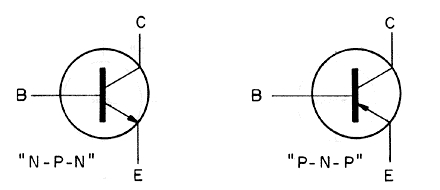
\includegraphics[scale=0.75]{imagenes/transistor.jpg}
\caption{Esquema transistores}
\end{figure}
\footnote{Universidad Politécnica de la Zona Metropolitana de Guadalajara}

\newpage
\section{Transistores bipolares de unión (BJT)}
Se forman agregando una segunda región p o n a un diodo de union pn. Con dos regiones n y una p, se forman dos uniones, teniéndose asi un transistor NPN, y con dos regiones p  y una n, se forma un transistor PNP, como se ve en la figura posee tres terminales (colector,  emisor y base).\\
Formado por dos uniones PN con tres zonas cada una conectada a los terminales:C: Colector, la zona
central es la B: Base y E: Emisor. El Emisor está muy impurificado, la Base tiene una impurificación
muy baja, mientras que el Colector posee una impurificación intermedia. Un transistor es similar a dos diodos, el transistor tiene dos uniones: una entre el emisor y la base y la otra entre la base y el colector.\\ El emisor y la base forman uno de los diodos, mientras que el colector y la base forman el otro. Estos diodos son denominados: "Diodo de emisor" (el de la izquierda en este caso) y "Diodo de colector" (el de la derecha en este caso). \\

\subsection{Ecuaciones de un circuito con transistor bipolar BJT}
\begin{figure}[hbtp]
\centering
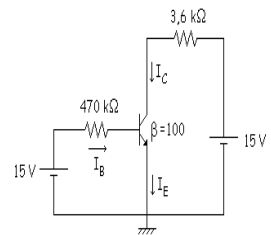
\includegraphics[scale=1]{imagenes/circuito.PNG}
\caption{Circuito con BJT}
\end{figure}

Ecuación de la malla de base:\\
$ VBE = 0.7V $
\begin{equation}
15 = 470*IB + VBE
\end{equation}
\begin{equation}
IB = \frac{15 - 0.7V}{3.6} = 30.4\mu A
\end{equation}

Ecuación de la malla del colector:\\
$  VCEsat = 0.2V $
\begin{equation}
15 = 3.6IC + VCE
\end{equation}
\begin{equation}
ICSAT = \frac{15 - 0.2V}{3.6} = 4.11\mu A
\end{equation}

Potencia máxima del transistor:\\
\begin{equation}
\textbf{Potencia disipada por un transistor:}
Pc = VCE * IC
\end{equation}
\begin{equation}
\textbf{Punto de trabajo óptimo:}
Pc = VCEQ = \frac{VCC}{2};
\end{equation}
\begin{equation}
ICQ = \frac{VCC}{2Rc}
\end{equation}
\footnote{Universidad Politécnica de la Zona Metropolitana de Guadalajara}

\newpage
\section{Transistores Efecto de campo (FET)}
 El transistor de efecto campo (Field-Effect Transistor o FET, en inglés) es en realidad una familia detransistores que se basan en el campo eléctrico para controlar la conductividad de un "canal" en un material semiconductor. Los FET pueden plantearse como resistencias controladas por diferencia de potencial.\\
Tienen tres terminales, denominadas puerta (gate), drenador (drain) y fuente (source). La puerta es la terminal equivalente a la base del BJT. El transistor de efecto de campo se comporta como un interruptor controlado por tensión, donde el voltaje aplicado a la puerta permite hacer que fluya o no corriente entre drenador y fuente.\\
\begin{figure}[hbtp]
\centering
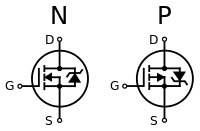
\includegraphics[scale=0.75]{imagenes/JFET.png}
\caption{Estrctura FET}
\end{figure}

Los transistores de efecto de campo o FET (Field Electric Transistor) son particularmente interesantes
en circuitos integrados y pueden ser de dos tipos:\\
\begin{itemize}
\item Transistor de efecto de campo de unión o JFET.
\item Transistor de efecto de campo metal-óxido semiconductor (MOSFET).
\end{itemize}

\subsection{JFET}
\textbf{Región corte}
\begin{equation}
pinch-off = VGS (off) o Vp
\end{equation}
\textbf{Región lineal}
\begin{equation}
I'DS(on) = \frac{1}{ID} [VDS - (\frac{2}{3}((\frac{VDS - VGS}{|Vp|^\frac{-1}{2}})^\frac{3}{2}) - \frac{VGS(^\frac{3}{2}}{|Vp|^\frac{1}{2}}]
\end{equation}
\textbf{Región saturación}
\begin{equation}
ID = IDSS (1 - \frac{VGS}{Vp}^2
\end{equation}

\subsection{MOSFET} 
\textbf{Región corte}
\begin{equation}
\textbf{Condición:} VGS<VTH
\end{equation}
\begin{equation}
\textbf{Intensidad:} ID = 0
\end{equation}
\textbf{Región lineal}
\begin{equation}
\textbf{Condiciones:} VGS>VTH\\
VGD<VTH VGS<VTH+VDS\\
\end{equation}
\begin{equation}
\textbf{Intensidad:} ID = k(VGS - VTH - \frac{VDS}{2})VDS
\end{equation}
\footnote{Universidad Politécnica de la Zona Metropolitana de Guadalajara}

\newpage
\section{Transistores bipolares de compuerta aislada  (IGBT).}
La sigla IGBT corresponde a las iniciales de isolated gate bipolar transistor o sea transistor bipolar de puerta de la salida. El IGBT es un dispositivo semiconductor de potencia híbrido que combina los atributos del TBJ y del MOSFET. Posee una compuerta tipo MOSFET y por consiguiente tiene una alta impedancia de entrada. El gate maneja voltaje como el MOSFET. El símbolo más comúnmente usado se muestra en la figura . Al igual que el MOSFET de potencia, el IGBT no exhibe el fenómeno de ruptura secundario como el TBJ.\\
El transistor bipolar de puerta aislada (IGBT) es un dispositivo electrónico que generalmente se aplica a circuitos de potencia. Este es un dispositivo para la conmutación en sistemas de alta tensión. La tensión de control de puerta es de unos 15V. Esto ofrece la ventaja de controlar sistemas de potencia aplicando una señal eléctrica de entrada muy débil en la puerta.\\
El IGBT de la figura es una conexión integrada de un MOSFET y un BJT. El circuito de excitación del IGBT es como el del MOSFET, mientras que las características de conducción son como las del BJT. El IGBT es adecuado para velocidades de conmutación de hasta 20 KHz y ha sustituido al BJT en muchas aplicaciones.\\
\begin{figure}[hbtp]
\centering
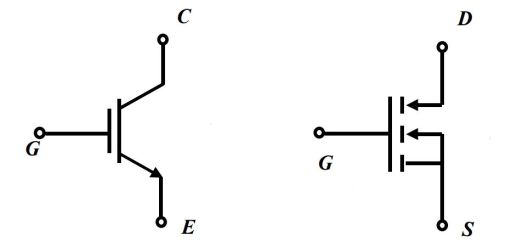
\includegraphics[scale=0.5]{imagenes/igbt.jpg}
\caption{Estructura del IGBT}
\end{figure}

\begin{equation}
VDS(on) =  VJI + IDR canal + IDR arrastre
\end{equation}
\begin{equation}
VJI = 0.7 + 1Volt
\end{equation}
\begin{equation}
R canal = R canal(MOS)
\end{equation}
\begin{equation}
R arrastre(IGBT) << R arrastre (MOS)
\end{equation}

\textbf{IGBT}
\begin{equation}
Voltaje = 1400V a 600V
\end{equation}
\begin{equation}
Corriente = 300A a 50A
\end{equation}
\footnote{Universidad Politécnica de la Zona Metropolitana de Guadalajara}

\newpage
\section{Referencias bibliográficas}

\url{http://www.iuma.ulpgc.es/~roberto/asignaturas/EI/transparencias/EI_Tema_3.2.Transistor_potencia.pdf}\\

\url{http://www.ele-mariamoliner.dyndns.org/~jsalgado/analogica/7transistores.pdf}\\

\url{https://sites.google.com/site/transistoresfototransistores/classroom-news}\\

\url{http://www.gte.us.es/~leopoldo/Store/tsp_6.pdf}\\


\end{document}